\subsection{Metodologia}

% \begin{frame}
%     \frametitle{Metodologia}
%     \framesubtitle{Treinamento dos AMs}
%     \begin{center}
%         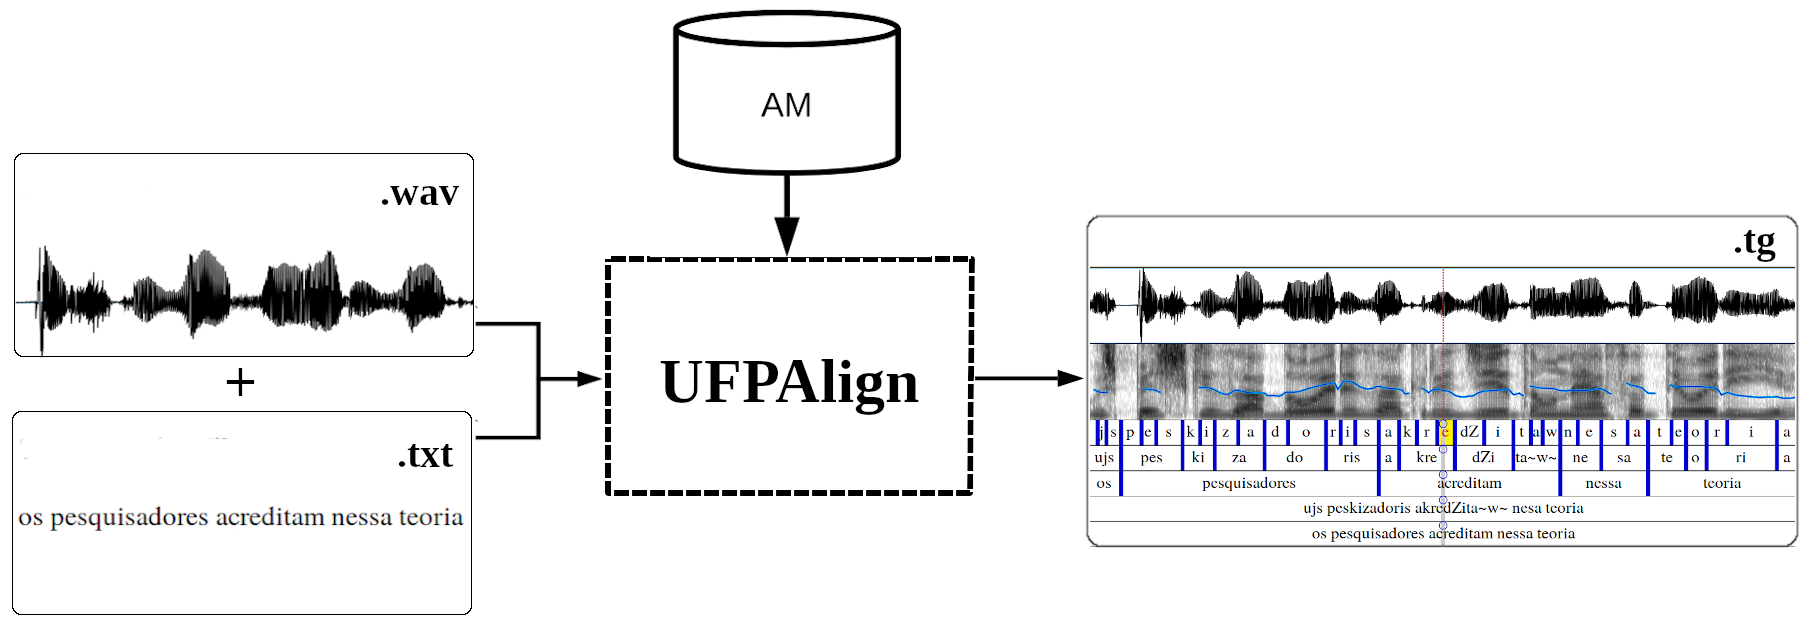
\includegraphics[width=1\textwidth]{Figures/ufpalign_geral}
%     \end{center}
% \end{frame}

\begin{frame}
    \frametitle{Metodologia}
    \framesubtitle{Base de \'Audio Transcrita}
    \begin{center}
        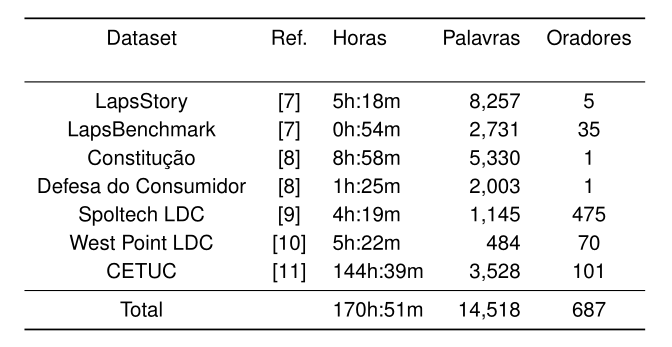
\includegraphics[width=0.8\textwidth]{Figures/db}
    \end{center}
\end{frame}

\begin{frame}
    \frametitle{Metodologia}
    \framesubtitle{Treinamento dos AMs}
    \begin{center}
        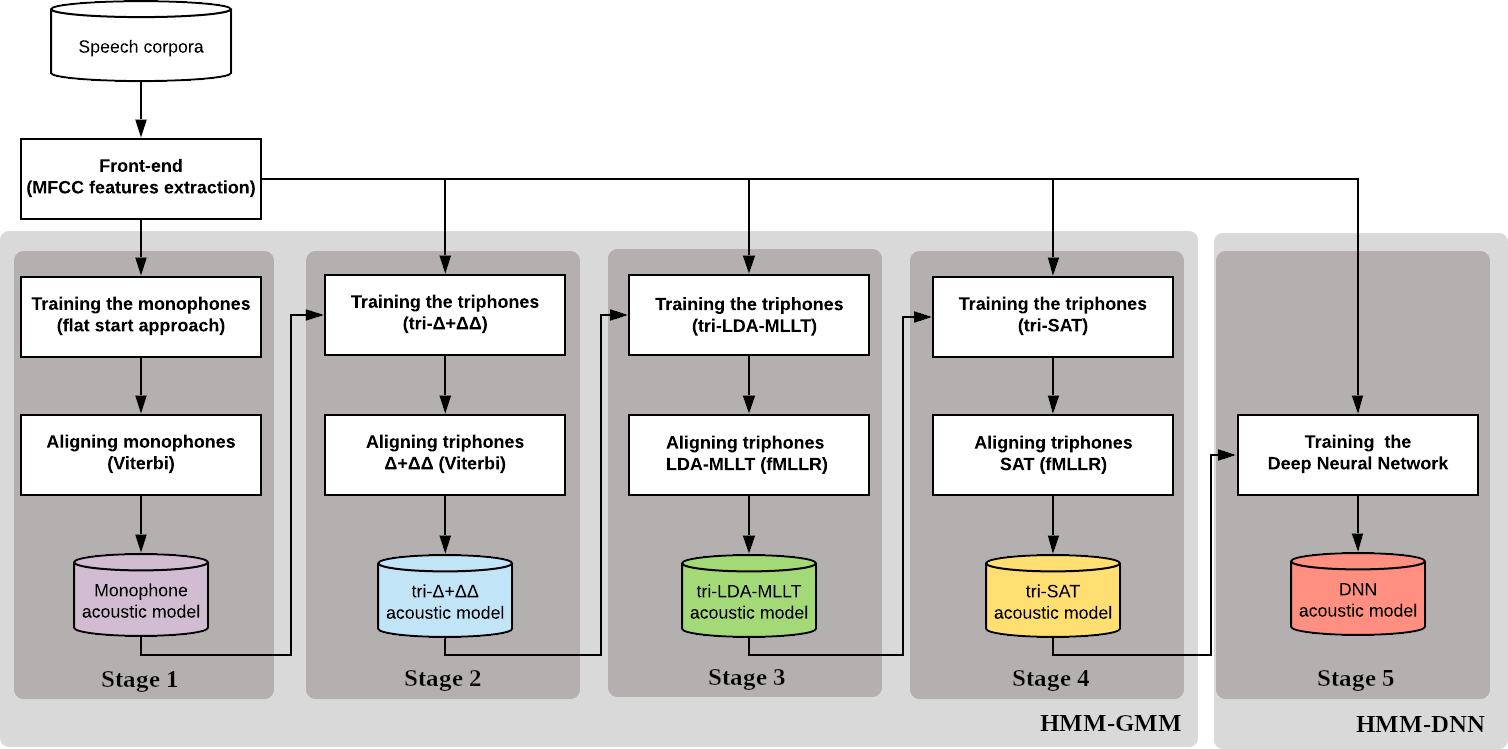
\includegraphics[width=1\textwidth]{Figures/kaldi_pipeline}
    \end{center}
\end{frame}

\begin{frame}
    \frametitle{Testes}
    \begin{itemize}
        \item \textit{Dataset} de Avalia\c c\~ao
        \begin{itemize}
            \item \'Audios de enunciados separados entre um locutor masculino (M) e um feminino
                (F)
            \item Arquivos \textit{TextGrid} de cada \'audio alinhados
                manualmente por um foneticista
        \end{itemize}
        \item Caracter\'istica comparada: limite fon\'etico
        \begin{itemize}
            \item Diferen\c ca entre o tempo final da ocorr\^encia do fonema em ambos alinhamentos, pelo alinhador e alinhado manualmente
        \end{itemize}
    \end{itemize}
\end{frame}
